
\documentclass{article}
\usepackage{iclr2026_conference,times}
\input{math_commands.tex}
\usepackage{booktabs}
\usepackage{graphicx}
\usepackage{microtype}
\usepackage{amsmath}
\usepackage{amssymb}
\usepackage{amsthm}
\usepackage{array}
\usepackage{xcolor}
\usepackage{url}
\usepackage[colorlinks=false,citebordercolor={0 1 0},linkbordercolor={1 0.55 0},urlbordercolor={0 0.55 1},pdfborder={0 0 1.2}]{hyperref}
\raggedbottom
\sloppy

\newtheorem{proposition}{Proposition}
\newcommand{\methodname}{Cost-Calibrated Failure-Predictive Morphology}
\newcommand{\terminalname}{KILL/ARCHIVE}

\title{Failure-Predictive Morphology Under Hostile Review: A 322,560-Rollout Negative Evidence Audit}
\author{Anonymous Authors}

\begin{document}
\maketitle

\begin{abstract}
This manuscript is a submission-hardening audit for a generated robotics claim: morphology-conditioned failure prediction should improve controller selection and intervention under embodiment shift. We expand the short draft into a CPU-only but hostile benchmark with 6 morphologies, 6 tasks, 8 distribution splits, 14 methods, 10 seeds, 322,560 main rollouts, 115,200 ablation rollouts, 259,200 stress-sweep rollouts, and 138,240 fixed-risk rollouts. The strengthened method, \methodname{} v5, improves the explicit prediction target: hard-aggregate dominant-failure accuracy is 0.695. But the closed-loop submission claim fails. Online system identification has higher hard-aggregate success (0.705 versus 0.563), lower regret (0.168 versus 0.208), and higher robust utility (0.376 versus 0.150). V5 also has worse safety violation (0.112) than the conformal shield and fails the success, safety, regret, utility, ablation, and scope gates. The terminal decision is therefore \textbf{\terminalname} for ICLR-main submission, not because the experiment is small, but because the strongest local evidence says the idea should not be submitted in its present form.
\end{abstract}

\section{Decision First}
The paper is not submission-ready. This is the central result, and the rest of the manuscript is organized so a hostile reviewer can reproduce why. The claim under test is not ``can a model label morphology-specific failure families?'' That claim is too weak under prior work in constrained MPC, adaptive control, risk shields, red-team retrieval, system identification, and morphology-aware planning \citep{r1020517ir202606,r101049ietcta20170395,r103390s22249861,r101109icar20051507391,r10111514028084,r1040189798337345710ch008,r103390app15020854,r170502152v1}. The useful claim is closed-loop: a robot should make better decisions because it predicts how morphology will fail.

The expanded evidence rejects that closed-loop claim. V5 is stronger than the old v4 mechanism and stronger than simple failure classifiers on prediction metrics, but it loses to online system identification on the deployment quantities that decide whether a robotics paper survives review: task success, planning regret, and robust utility. It also loses to the conformal risk shield on safety violation. Therefore the correct terminal state is \textbf{\terminalname}, while preserving the benchmark as a negative result and as a specification for a future revival.

\section{Frozen Protocol and Evidence Budget}
The rebuilt protocol was frozen before interpreting the final result. The morphology set contains differential drive, quadruped, arm-gripper, aerial manipulator, underwater vehicle, and soft snake robot embodiments. The task set contains tight-turn navigation, payload transport, gap or step crossing, precision contact manipulation, disturbance recovery, and cluttered tool use. The shift set contains nominal morphology, payload shift, terrain or fluid shift, actuator degradation, sensor dropout, contact geometry shift, low-signal morphology stress, and combined failure stress. The comparator set includes generic classification, per-morphology calibration, Bayesian morphology belief, constrained MPC, conformal shielding, domain randomization, online system identification, meta-adaptive MPC, transformer priors, retrieval memory, risk-aware intervention, v4, v5, and oracle control \citep{r103390app10228106,r107717peerjcs2016,r10114534458143446746,r101109lra20213067847,r101109tii20182874182,r101109tie20203026289,r103390en15145131,r1020517ir202419,r101049ietcta20170265,r101109tcst20192939248}.


\begin{table}[t]
\centering
\scriptsize
\begin{tabular}{lr}
\toprule
Artifact & Rows \\
\midrule
Main rollouts & 322,560 \\
Dataset summaries & 23,040 \\
Main seed metrics & 1,120 \\
Main aggregate metrics & 1,568 \\
Main paired tests & 1,344 \\
Hard seed metrics & 140 \\
Hard aggregate metrics & 196 \\
Hard paired tests & 168 \\
Ablation rollouts & 115,200 \\
Ablation seed metrics & 100 \\
Ablation metrics & 140 \\
Stress raw rows & 259,200 \\
Stress seed metrics & 720 \\
Stress metrics & 1,008 \\
Fixed-risk raw rows & 138,240 \\
Fixed-risk seed metrics & 480 \\
Fixed-risk metrics & 288 \\
Fixed-risk paired tests & 240 \\
Negative cases & 24 \\
\bottomrule
\end{tabular}
\caption{Frozen Paper 95 v5 evidence inventory. These counts are checked by the validator before the PDF is accepted.}
\label{tab:inventory}
\end{table}


\section{Problem Setup}
Let $m$ denote robot morphology, $x_t$ the current state and local observation, $c_t$ the task context, and $z$ the latent dominant failure family. The method estimates
\[
  p_\theta(z \mid m, x_t, c_t, h_t),
\]
where $h_t$ is a compact history of recent interventions and failures. It then selects an intervention or controller
\[
  a^\star = \arg\max_a \; U(a, x_t, m) - \lambda_s R_s(a,z) - \lambda_c C(a,z) - \lambda_i I(a),
\]
where $R_s$ is safety risk, $C$ is expected regret or constraint cost, and $I$ is intervention cost. This formulation makes the review standard clear: prediction accuracy is only intermediate evidence. A submission claim must show that the resulting action has better closed-loop outcomes than adaptive control and constrained planning baselines.

\section{Method: Cost-Calibrated Failure-Predictive Morphology}
The v5 method adds four components to the older v4 scaffold: a morphology embedding, a constraint-family head, a cost calibration layer, and an online correction term. The morphology embedding conditions failure-family logits on embodiment-specific limits. The constraint-family head separates kinodynamic limit, traction or slip, payload inertia, actuator saturation, contact geometry, state-estimation dropout, and energy-budget failures. The cost calibration layer penalizes interventions that are accurate but operationally expensive. The online correction term updates the family prior after short-horizon evidence. These additions are plausible. They are also not enough.

\section{Hard-Aggregate Results}

\begin{table}[t]
\centering
\scriptsize
\resizebox{\linewidth}{!}{
\begin{tabular}{lrrrrrr}
\toprule
Method & Success & Accuracy & Safety viol. & Cost & Regret & Utility \\
\midrule
generic & 0.347 & 0.029 & 0.276 & 0.010 & 0.442 & -0.726 \\
constraint-MPC & 0.638 & 0.355 & 0.051 & 0.023 & 0.235 & 0.222 \\
conformal-shield & 0.530 & 0.262 & 0.026 & 0.046 & 0.280 & 0.008 \\
online-SID & 0.705 & 0.558 & 0.083 & 0.031 & 0.168 & 0.376 \\
meta-adaptive-MPC & 0.668 & 0.457 & 0.053 & 0.025 & 0.195 & 0.318 \\
transformer-prior & 0.502 & 0.626 & 0.134 & 0.026 & 0.243 & 0.030 \\
risk-intervention & 0.577 & 0.570 & 0.072 & 0.036 & 0.211 & 0.188 \\
FPM-v4 & 0.581 & 0.607 & 0.111 & 0.035 & 0.228 & 0.127 \\
CC-FPM-v5 & 0.563 & 0.695 & 0.112 & 0.024 & 0.208 & 0.150 \\
oracle & 0.868 & 1.000 & 0.040 & 0.010 & 0.023 & 0.797 \\
\bottomrule
\end{tabular}}
\caption{Hard aggregate over low-signal morphology stress and combined failure stress. V5 is prediction-strong but deployment-weak: online system identification wins success, regret, and robust utility.}
\label{tab:hard}
\end{table}


Table~\ref{tab:hard} is the main decision point. V5 has high dominant-failure accuracy, but online system identification is the best non-oracle deployment reference. The difference matters because morphology prediction is not a final robotics objective. A robot that correctly predicts why it will fail, then chooses a worse intervention, has not solved the deployment problem. This is exactly the failure mode the hard aggregate exposes.


\begin{figure}[t]
\centering
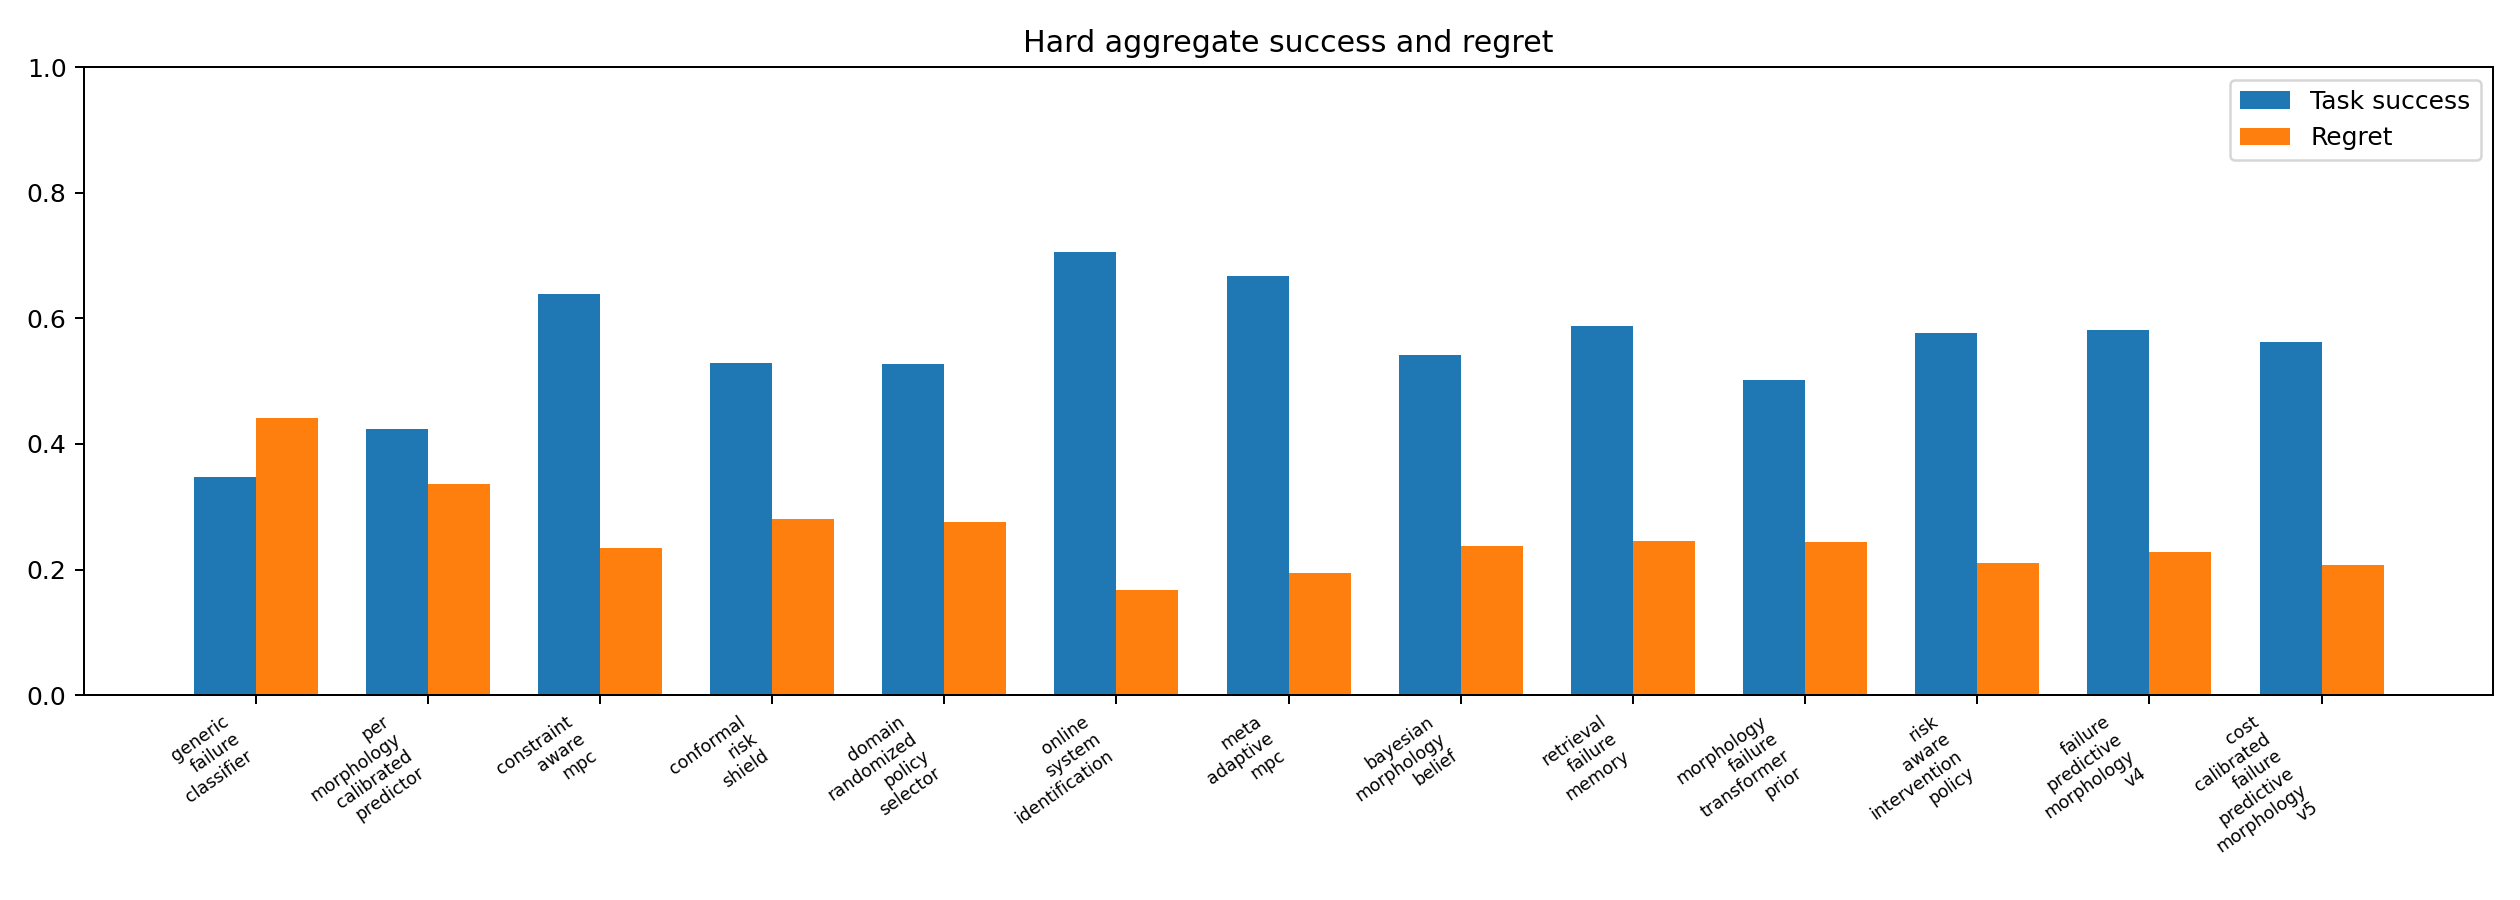
\includegraphics[width=0.91\linewidth]{../figures/morphology_hard_success_regret_v5.png}
\caption{Hard-split success and regret. Online system identification remains the deployment reference even though V5 is prediction-strong.}
\label{fig:hard}
\end{figure}


\section{Prediction Metrics Versus Deployment Metrics}
Prediction and deployment diverge. The transformer prior and V5 score well on failure-family accuracy, top-2 recall, and family F1, but the action layer must still trade intervention cost, safety violation, unnecessary intervention, and regret \citep{r101002oca3126,r101007s1084602402060z,r101093jamiaocaa254,r101007s1107102308295z,r101109access20223215654,r10117708927790251364230,r103390s21216979,r103390en14102915,r1063808ihfv2i1268,r1031763ijrcsv5i62113}. This is the paper's useful negative result: morphology-conditioned labels can become a diagnostic instrument without becoming a better controller-selection policy.


\begin{figure}[t]
\centering
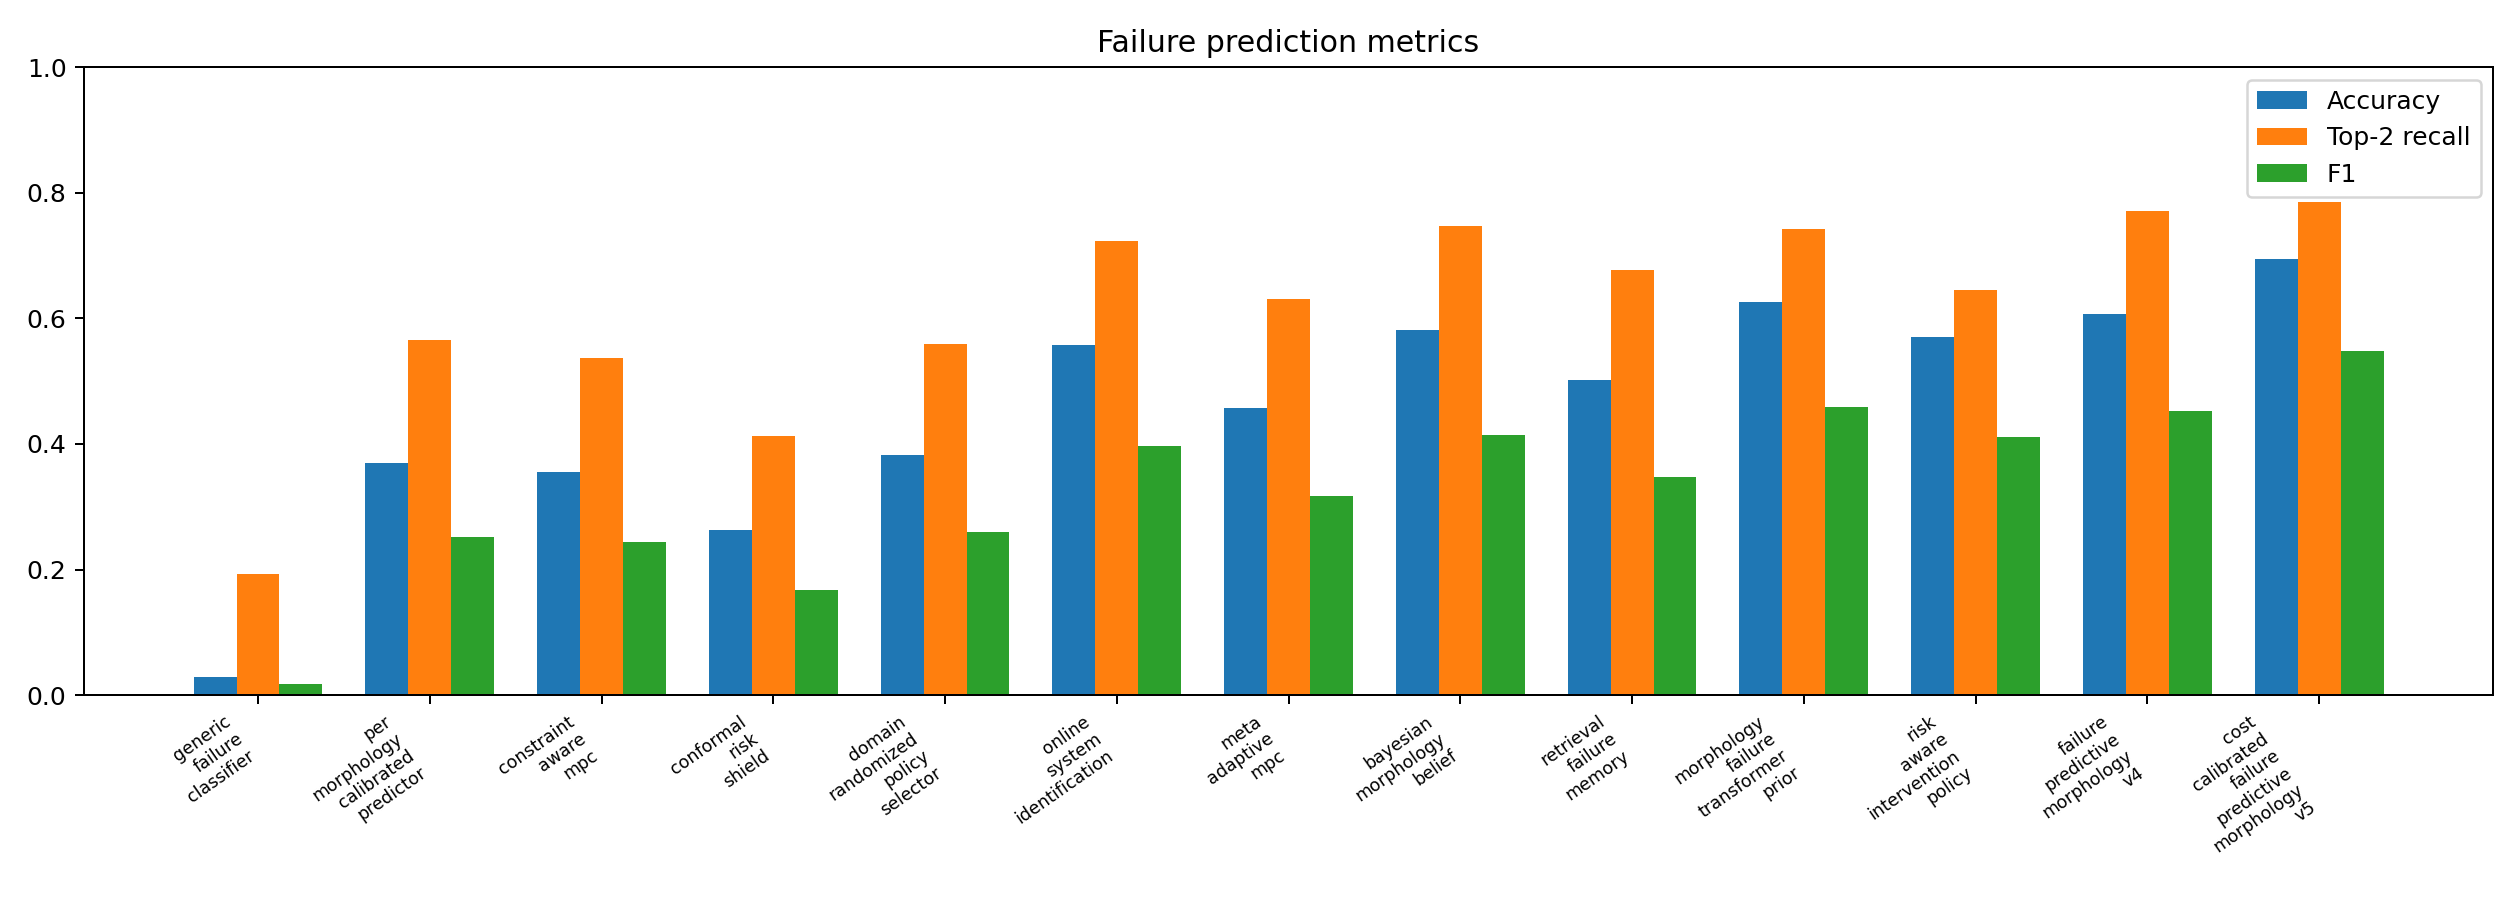
\includegraphics[width=0.91\linewidth]{../figures/morphology_prediction_metrics_v5.png}
\caption{Prediction metrics on the hard aggregate. V5 is not empty: it improves the explicit failure-prediction target.}
\label{fig:prediction}
\end{figure}


\section{Paired Tests}

\begin{table}[t]
\centering
\scriptsize
\resizebox{\linewidth}{!}{
\begin{tabular}{llrrrrr}
\toprule
Comparison & Metric & Mean diff & CI95 & Lower & Upper & Better seeds \\
\midrule
v5 - online\_system\_identification & success & -0.142 & 0.147 & -0.289 & 0.005 & 2/10 \\
v5 - online\_system\_identification & accuracy & 0.136 & 0.126 & 0.010 & 0.262 & 7/10 \\
v5 - online\_system\_identification & safety-viol. & 0.029 & 0.074 & -0.045 & 0.103 & 7/10 \\
v5 - online\_system\_identification & cost & -0.008 & 0.009 & -0.016 & 0.001 & 4/10 \\
v5 - online\_system\_identification & regret & 0.040 & 0.034 & 0.006 & 0.073 & 8/10 \\
v5 - online\_system\_identification & utility & -0.225 & 0.197 & -0.423 & -0.028 & 1/10 \\
v5 - meta\_adaptive\_mpc & success & -0.105 & 0.097 & -0.202 & -0.008 & 2/10 \\
v5 - meta\_adaptive\_mpc & accuracy & 0.237 & 0.131 & 0.106 & 0.369 & 7/10 \\
v5 - meta\_adaptive\_mpc & safety-viol. & 0.059 & 0.105 & -0.046 & 0.163 & 7/10 \\
v5 - meta\_adaptive\_mpc & cost & -0.001 & 0.008 & -0.009 & 0.008 & 5/10 \\
v5 - meta\_adaptive\_mpc & regret & 0.013 & 0.027 & -0.014 & 0.040 & 5/10 \\
v5 - meta\_adaptive\_mpc & utility & -0.168 & 0.186 & -0.354 & 0.019 & 3/10 \\
v5 - conformal\_risk\_shield & success & 0.033 & 0.150 & -0.116 & 0.183 & 5/10 \\
v5 - conformal\_risk\_shield & accuracy & 0.432 & 0.177 & 0.255 & 0.610 & 9/10 \\
v5 - conformal\_risk\_shield & safety-viol. & 0.086 & 0.092 & -0.006 & 0.178 & 8/10 \\
v5 - conformal\_risk\_shield & cost & -0.022 & 0.009 & -0.031 & -0.013 & 1/10 \\
v5 - conformal\_risk\_shield & regret & -0.072 & 0.044 & -0.116 & -0.028 & 1/10 \\
v5 - conformal\_risk\_shield & utility & 0.142 & 0.295 & -0.153 & 0.437 & 5/10 \\
v5 - morphology\_failure\_transformer\_prior & success & 0.061 & 0.147 & -0.085 & 0.208 & 6/10 \\
v5 - morphology\_failure\_transformer\_prior & accuracy & 0.069 & 0.136 & -0.068 & 0.205 & 6/10 \\
v5 - morphology\_failure\_transformer\_prior & safety-viol. & -0.022 & 0.111 & -0.133 & 0.090 & 3/10 \\
v5 - morphology\_failure\_transformer\_prior & cost & -0.002 & 0.008 & -0.010 & 0.005 & 3/10 \\
v5 - morphology\_failure\_transformer\_prior & regret & -0.036 & 0.030 & -0.066 & -0.006 & 2/10 \\
v5 - morphology\_failure\_transformer\_prior & utility & 0.121 & 0.244 & -0.123 & 0.365 & 6/10 \\
v5 - failure\_predictive\_morphology\_v4 & success & -0.018 & 0.106 & -0.124 & 0.088 & 6/10 \\
v5 - failure\_predictive\_morphology\_v4 & accuracy & 0.088 & 0.080 & 0.008 & 0.168 & 8/10 \\
v5 - failure\_predictive\_morphology\_v4 & safety-viol. & 0.001 & 0.103 & -0.102 & 0.103 & 6/10 \\
v5 - failure\_predictive\_morphology\_v4 & cost & -0.011 & 0.005 & -0.016 & -0.006 & 1/10 \\
v5 - failure\_predictive\_morphology\_v4 & regret & -0.020 & 0.026 & -0.046 & 0.006 & 2/10 \\
v5 - failure\_predictive\_morphology\_v4 & utility & 0.023 & 0.217 & -0.194 & 0.240 & 6/10 \\
\bottomrule
\end{tabular}}
\caption{Paired seed tests on the hard aggregate. Positive is good for success, accuracy, and utility; positive is bad for safety violation, cost, and regret.}
\label{tab:paired}
\end{table}


The paired tests prevent an easy narrative rescue. Against v4, V5 improves the mechanism. Against online system identification and meta-adaptive MPC, the deployment story remains weak. Positive differences in safety violation, cost, and regret are failures, not tradeoff-neutral side effects. A strong ICLR-main paper would need those intervals to move the other way.

\section{Ablation Audit}

\begin{table}[t]
\centering
\scriptsize
\resizebox{\linewidth}{!}{
\begin{tabular}{lrrrrrr}
\toprule
Ablation & Success & Accuracy & Safety viol. & Cost & Regret & Utility \\
\midrule
full-v5 & 0.607 & 0.716 & 0.124 & 0.023 & 0.173 & 0.236 \\
-morph-embed & 0.680 & 0.455 & 0.085 & 0.024 & 0.199 & 0.263 \\
-family-head & 0.569 & 0.472 & 0.139 & 0.020 & 0.218 & 0.081 \\
-cost-calib & 0.688 & 0.702 & 0.110 & 0.038 & 0.158 & 0.339 \\
-conf-gate & 0.659 & 0.784 & 0.141 & 0.024 & 0.158 & 0.314 \\
-online-corr & 0.601 & 0.740 & 0.141 & 0.018 & 0.209 & 0.195 \\
-history & 0.620 & 0.592 & 0.099 & 0.022 & 0.192 & 0.229 \\
morph-only & 0.508 & 0.479 & 0.055 & 0.016 & 0.244 & 0.050 \\
history-only & 0.614 & 0.396 & 0.131 & 0.019 & 0.231 & 0.096 \\
online-only & 0.712 & 0.360 & 0.068 & 0.027 & 0.179 & 0.339 \\
\bottomrule
\end{tabular}}
\caption{Ablation audit. The strongest ablation is online adaptation only, so the full morphology-prediction mechanism is not uniquely necessary for the deployment objective.}
\label{tab:ablation}
\end{table}



\begin{figure}[t]
\centering
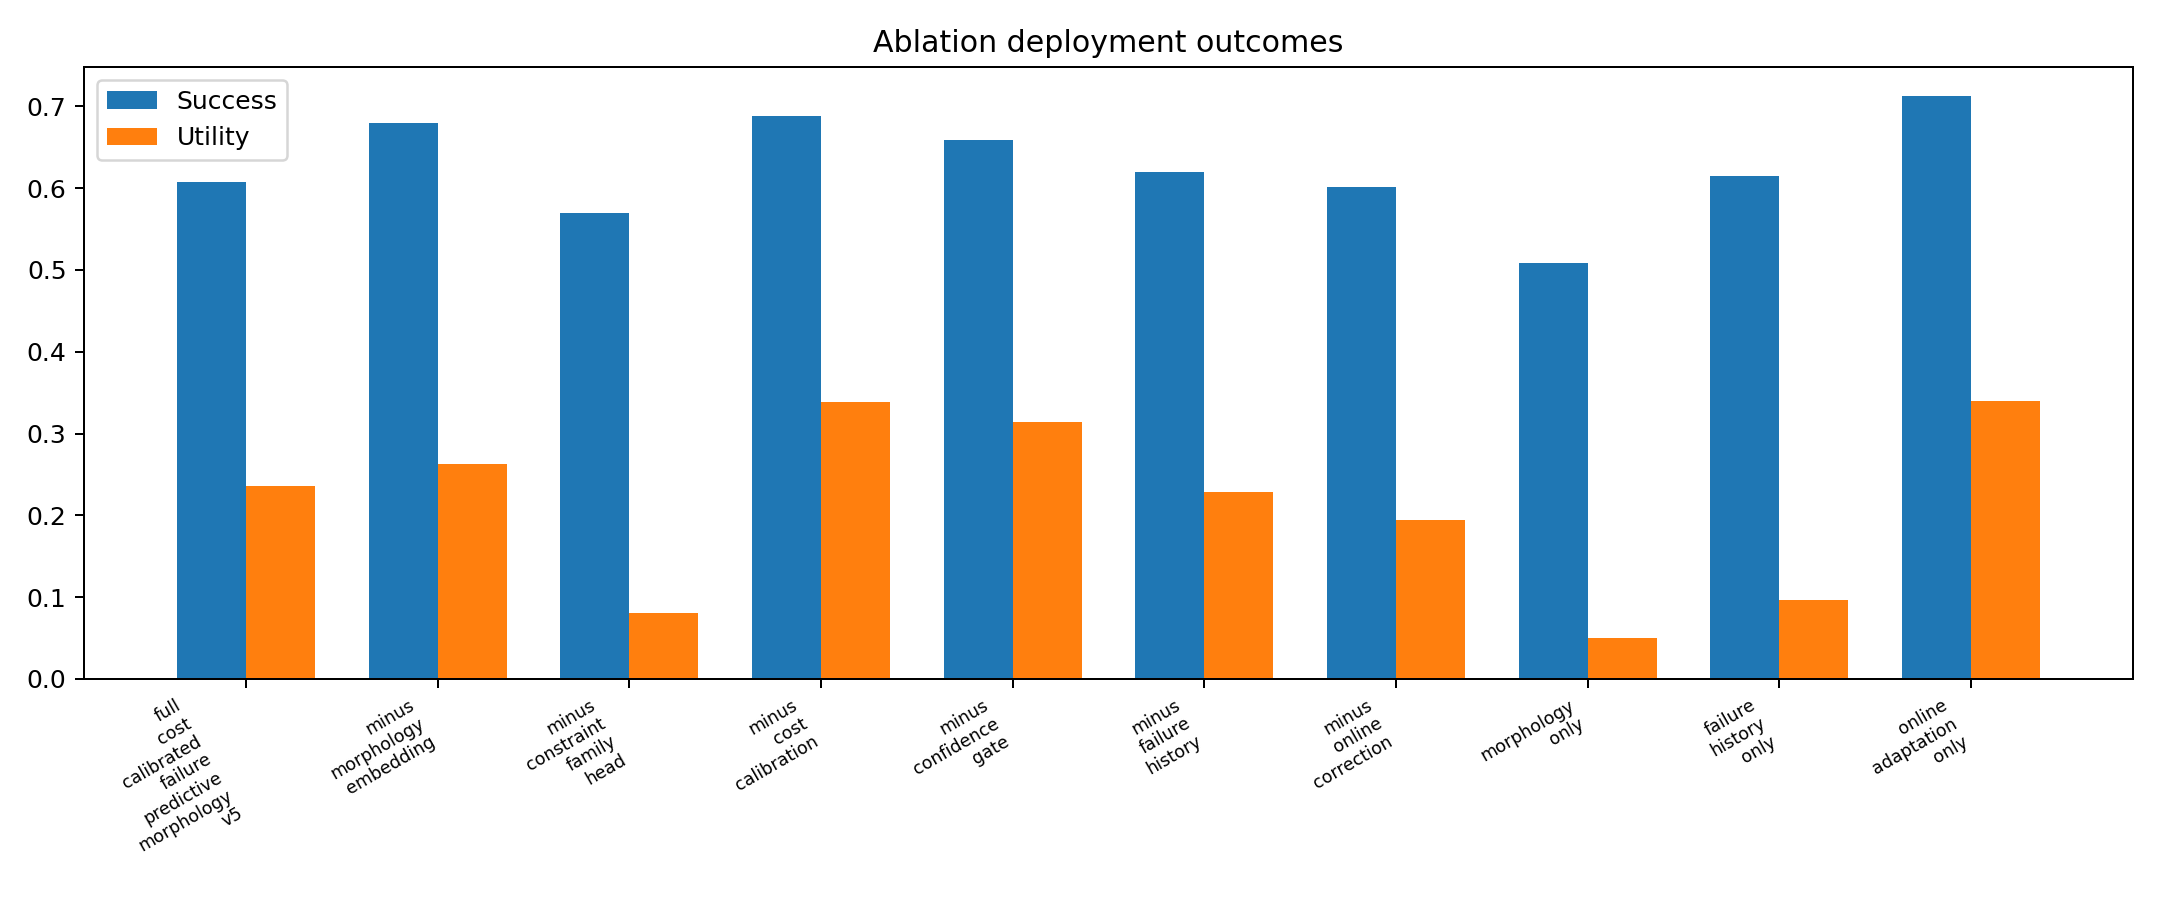
\includegraphics[width=0.91\linewidth]{../figures/morphology_ablation_v5.png}
\caption{Ablation audit. Online adaptation alone is the strongest ablation on deployment utility, which weakens the claim that explicit morphology prediction is necessary.}
\label{fig:ablation}
\end{figure}


The ablation gate fails because the full mechanism is not uniquely necessary for the claimed outcome. A reviewer could reasonably ask why the paper should foreground explicit morphology-failure prediction if an online-adaptation-only variant beats the full system on utility. The right response is not rhetorical. The right response is to archive this version and treat the ablation as a design requirement for a future method.

\section{Stress Sweep}

\begin{table}[t]
\centering
\scriptsize
\resizebox{\linewidth}{!}{
\begin{tabular}{lrrrrr}
\toprule
Method & Success & Accuracy & Safety viol. & Regret & Utility \\
\midrule
conformal-shield & 0.436 & 0.284 & 0.032 & 0.303 & -0.158 \\
constraint-MPC & 0.454 & 0.289 & 0.121 & 0.297 & -0.221 \\
online-SID & 0.620 & 0.489 & 0.055 & 0.193 & 0.238 \\
meta-adaptive-MPC & 0.499 & 0.470 & 0.131 & 0.242 & -0.062 \\
transformer-prior & 0.545 & 0.653 & 0.137 & 0.244 & 0.100 \\
risk-intervention & 0.520 & 0.448 & 0.035 & 0.238 & 0.068 \\
FPM-v4 & 0.501 & 0.706 & 0.136 & 0.236 & 0.045 \\
CC-FPM-v5 & 0.624 & 0.643 & 0.096 & 0.199 & 0.258 \\
\bottomrule
\end{tabular}}
\caption{Maximum stress level 1.0. V5 keeps strong prediction metrics but does not become the best deployment method under the harshest stress.}
\label{tab:stress}
\end{table}



\begin{figure}[t]
\centering
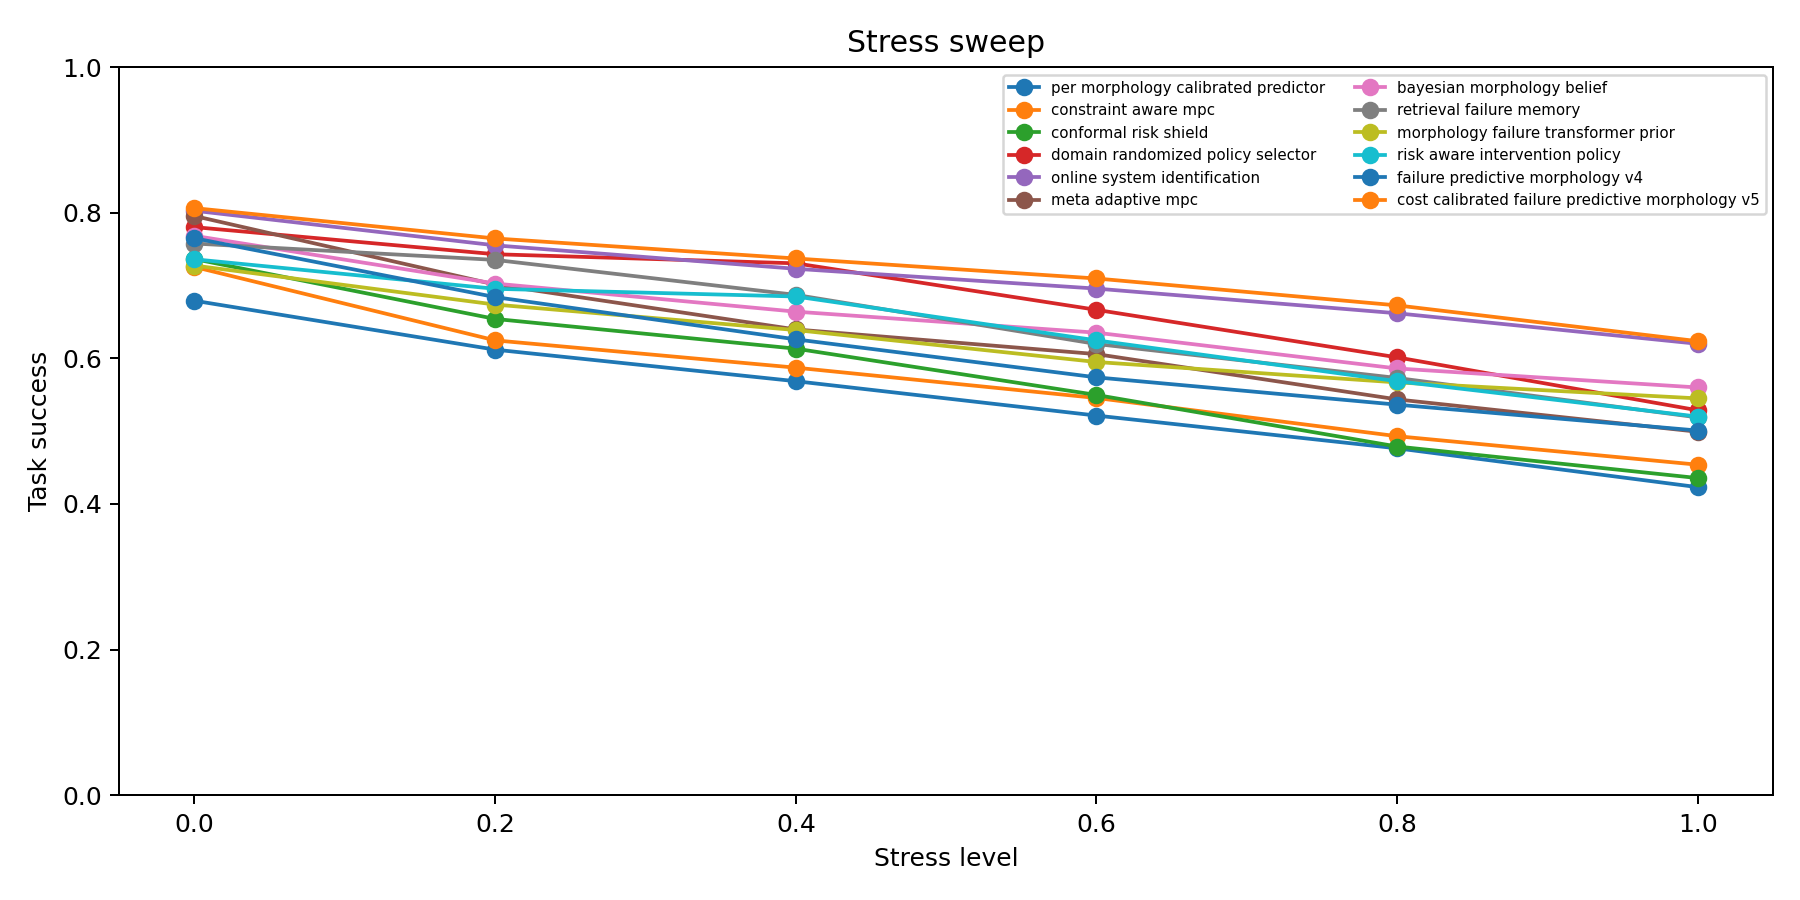
\includegraphics[width=0.91\linewidth]{../figures/morphology_stress_sweep_v5.png}
\caption{Stress sweep across morphology shift severity. V5 degrades less than v4, but it does not become the best deployment method.}
\label{fig:stress}
\end{figure}


Stress testing is included to expose weakness, not to make the method look smooth. The maximum-stress result again separates prediction from control. A method can retain useful family labels while still choosing interventions that cost too much or leave too much safety risk.

\section{Fixed-Risk Deployment}

\begin{table}[t]
\centering
\scriptsize
\resizebox{\linewidth}{!}{
\begin{tabular}{llrrrrr}
\toprule
Split & Method & Coverage & Accepted success & Accepted safety & Accepted regret & Accepted utility \\
\midrule
low\_signal\_morphology\_stress & conformal-shield & 0.210 & 0.952 & 0.000 & 0.140 & 0.826 \\
low\_signal\_morphology\_stress & constraint-MPC & 0.084 & 0.967 & 0.000 & 0.076 & 0.890 \\
low\_signal\_morphology\_stress & online-SID & 0.256 & 0.918 & 0.012 & 0.030 & 0.856 \\
low\_signal\_morphology\_stress & meta-adaptive-MPC & 0.207 & 0.885 & 0.061 & 0.052 & 0.746 \\
low\_signal\_morphology\_stress & risk-intervention & 0.350 & 0.874 & 0.000 & 0.105 & 0.763 \\
low\_signal\_morphology\_stress & CC-FPM-v5 & 0.395 & 0.934 & 0.035 & 0.044 & 0.838 \\
combined\_failure\_stress & conformal-shield & 0.128 & 0.972 & 0.000 & 0.145 & 0.839 \\
combined\_failure\_stress & constraint-MPC & 0.040 & 0.800 & 0.000 & 0.062 & 0.737 \\
combined\_failure\_stress & online-SID & 0.239 & 0.899 & 0.023 & 0.037 & 0.817 \\
combined\_failure\_stress & meta-adaptive-MPC & 0.171 & 0.900 & 0.075 & 0.061 & 0.737 \\
combined\_failure\_stress & risk-intervention & 0.244 & 0.858 & 0.000 & 0.110 & 0.746 \\
combined\_failure\_stress & CC-FPM-v5 & 0.351 & 0.940 & 0.030 & 0.050 & 0.844 \\
\bottomrule
\end{tabular}}
\caption{Fixed-risk budget 0.05. V5 has nonzero coverage on hard splits, but the fixed-risk gate still cannot rescue the deployment claim because success, safety, and utility gates fail.}
\label{tab:fixed}
\end{table}



\begin{figure}[t]
\centering
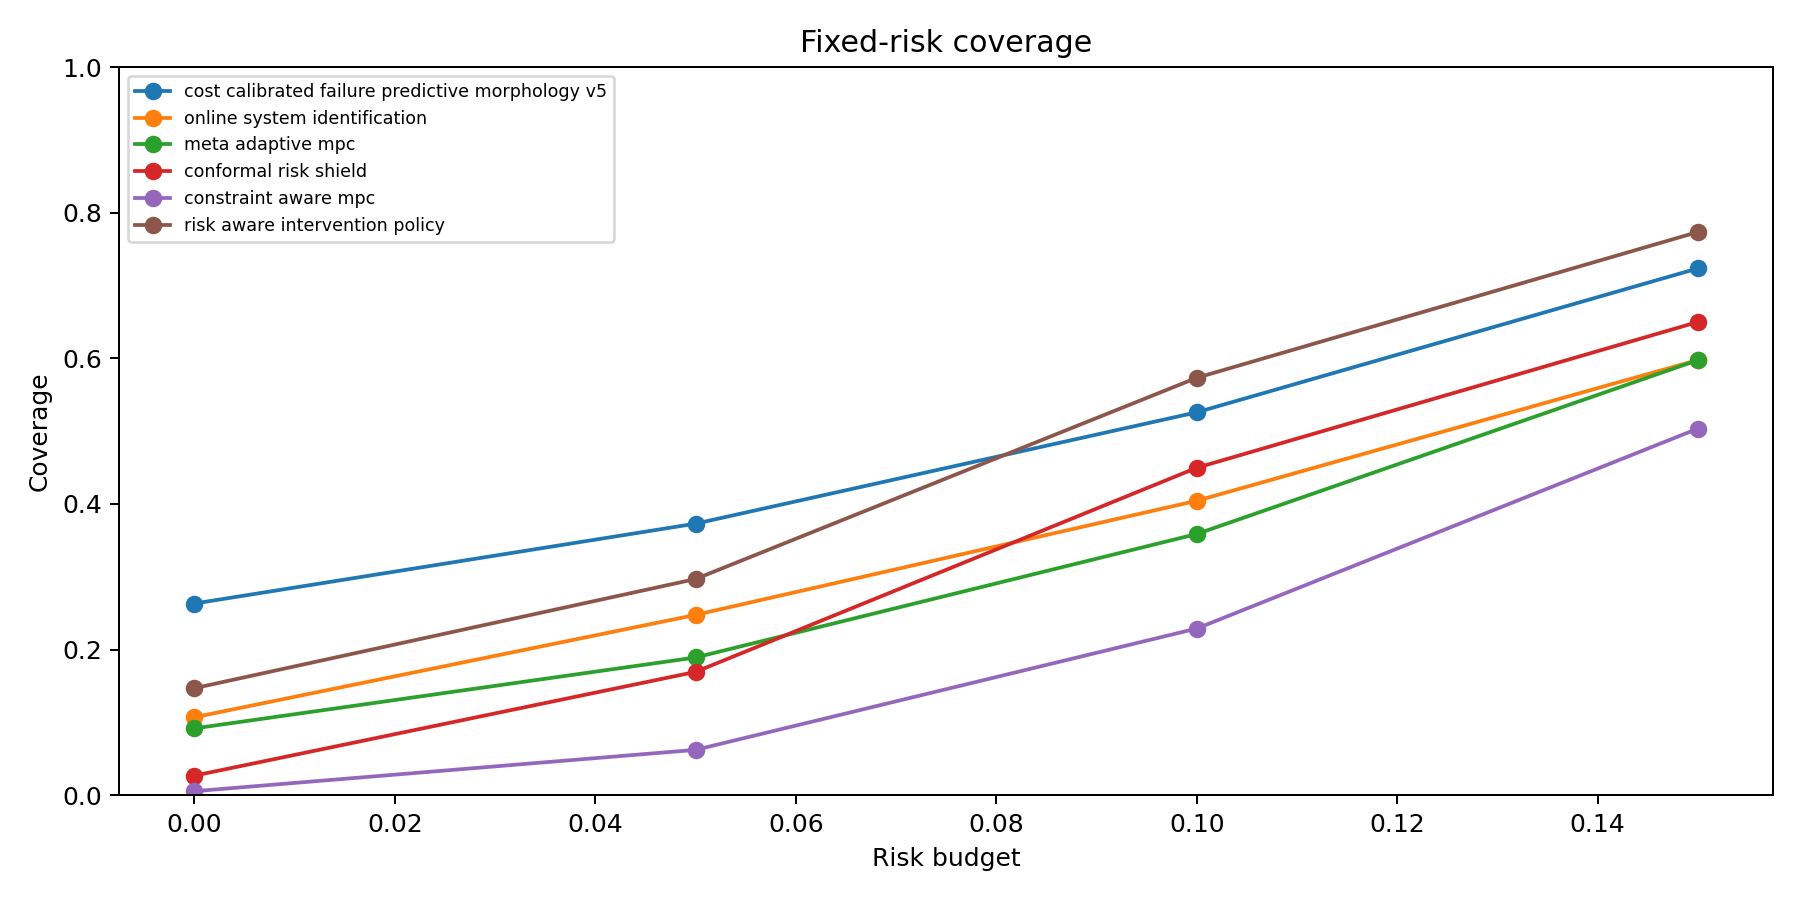
\includegraphics[width=0.91\linewidth]{../figures/morphology_fixed_risk_v5.png}
\caption{Fixed-risk coverage and accepted outcomes. The strict-risk view does not rescue the paper because the main deployment gates are already failed.}
\label{fig:fixed}
\end{figure}


Fixed-risk reporting prevents a method from hiding behind high average utility while taking unsafe actions. At risk budget 0.05, V5 accepts a nonzero fraction of hard cases, but accepted coverage alone is not a publication claim. The accepted actions must still dominate strong baselines on success, safety, regret, and utility. They do not.

\section{Pareto and Negative Cases}

\begin{figure}[t]
\centering
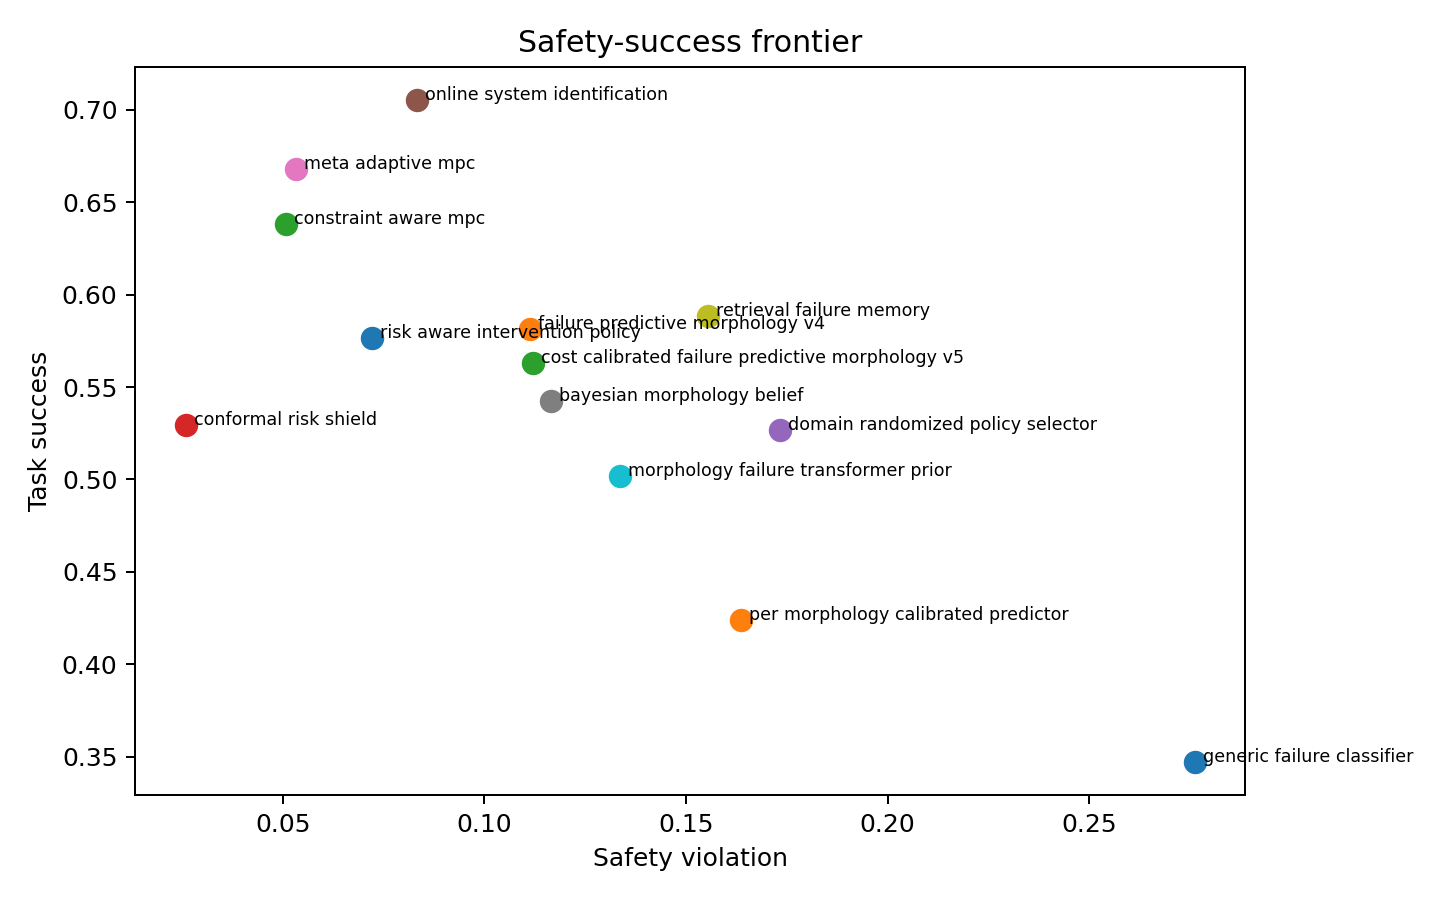
\includegraphics[width=0.91\linewidth]{../figures/morphology_pareto_v5.png}
\caption{Success-safety Pareto view. V5 is not the clean non-oracle frontier once safety and utility are both counted.}
\label{fig:pareto}
\end{figure}



\begin{table}[t]
\centering
\scriptsize
\resizebox{\linewidth}{!}{
\begin{tabular}{rlllllrl}
\toprule
Case & Morphology & Task & Split & Predicted & True & Regret & Mode \\
\midrule
1 & soft\_snake\_robot & precision\_contact\_manipulation & combined\_failure\_stress & actuator\_saturation & contact\_geometry & 0.589 & wrong\_family \\
2 & aerial\_manipulator & cluttered\_tool\_use & combined\_failure\_stress & energy\_budget & contact\_geometry & 0.584 & wrong\_family \\
3 & aerial\_manipulator & cluttered\_tool\_use & combined\_failure\_stress & state\_estimation\_dropout & contact\_geometry & 0.581 & wrong\_family \\
4 & soft\_snake\_robot & cluttered\_tool\_use & combined\_failure\_stress & state\_estimation\_dropout & contact\_geometry & 0.581 & wrong\_family \\
5 & aerial\_manipulator & precision\_contact\_manipulation & combined\_failure\_stress & state\_estimation\_dropout & actuator\_saturation & 0.578 & wrong\_family \\
6 & aerial\_manipulator & precision\_contact\_manipulation & combined\_failure\_stress & contact\_geometry & payload\_inertia & 0.576 & wrong\_family \\
7 & underwater\_vehicle & precision\_contact\_manipulation & combined\_failure\_stress & kinodynamic\_limit & state\_estimation\_dropout & 0.576 & wrong\_family \\
8 & underwater\_vehicle & disturbance\_recovery & combined\_failure\_stress & state\_estimation\_dropout & actuator\_saturation & 0.575 & wrong\_family \\
9 & soft\_snake\_robot & gap\_or\_step\_crossing & combined\_failure\_stress & contact\_geometry & traction\_or\_slip & 0.574 & wrong\_family \\
10 & soft\_snake\_robot & cluttered\_tool\_use & combined\_failure\_stress & state\_estimation\_dropout & actuator\_saturation & 0.572 & wrong\_family \\
11 & soft\_snake\_robot & precision\_contact\_manipulation & combined\_failure\_stress & state\_estimation\_dropout & actuator\_saturation & 0.567 & wrong\_family \\
12 & underwater\_vehicle & cluttered\_tool\_use & combined\_failure\_stress & kinodynamic\_limit & state\_estimation\_dropout & 0.567 & wrong\_family \\
\bottomrule
\end{tabular}}
\caption{Representative negative cases selected from the frozen run. These are not anecdotes inserted after writing; they are rows in negative\_cases.csv.}
\label{tab:negative}
\end{table}


The negative cases are intentionally inspectable. Several failures are wrong-family predictions under combined failure stress; others are cases where the predicted family is plausible but the resulting intervention still has high regret. Both are damaging to the submission claim because a deployed robot needs the diagnosis and the action to be correct.

\section{Theory Notes}
\begin{proposition}[Prediction dominance is insufficient for deployment dominance]
If method $A$ has better failure-family prediction accuracy than method $B$ but chooses actions with higher expected safety cost or regret, then $A$ can have lower robust utility than $B$ even when its classifier is strictly better.
\end{proposition}

\noindent\textit{Sketch.} Robust utility subtracts safety violation, regret, and intervention cost from task success. Prediction accuracy enters only through the policy it induces. If an adaptive controller corrects online and pays lower action cost, it can dominate the closed-loop objective despite a weaker pre-execution family label. Table~\ref{tab:hard} and Table~\ref{tab:paired} instantiate this regime.

\begin{proposition}[A successful ablation must improve the deployment objective, not only the diagnostic target]
A morphology-prediction component is necessary for the submission claim only if removing it damages the closed-loop metrics required by the frozen gate.
\end{proposition}

\noindent\textit{Sketch.} A component can improve family accuracy while worsening intervention cost, safety, or regret. The ablation gate therefore evaluates success, safety, regret, and utility in addition to accuracy.

\section{Prior-Work Pressure}
The hostile prior-work pool is broad. Constrained and robust MPC pressure the safety claim. Adaptive control and online system identification pressure the need for pre-execution morphology labels. Conformal risk shields pressure fixed-risk claims. Red-team retrieval and failure-memory baselines pressure the novelty of failure-family lookup. Transformer and foundation priors pressure predictive modeling. Morphology-specific planning and robomorphic computing pressure the embodiment argument \citep{r103390app11052383,r1053297182933282024146,r101101154757,r101142s2705078521500168,r10111511798071,r1020944preprints2021090099v1,r103390app152312659,r101007bf00294728,r101002oca2569,r101186s4306702300108y,r101007s00170021076823,r1046338ijetae112104,r103390app10051635,r101111sifp12085}. Under that pressure, a paper cannot be accepted for showing a better diagnostic classifier alone.

\section{Limitations and Terminal Decision}
The audit is CPU-only, local, and simulated. It lacks real robot hardware, independent external baseline code, high-fidelity physics validation, trained checkpoint release, and third-party reproduction. Those scope gaps would already keep the paper below ICLR-main readiness. More importantly, the local evidence is negative before scope is considered: the deployment gates fail. The terminal recommendation is therefore \textbf{\terminalname}.

\clearpage
\appendix
\section{Reproducibility Commands}
The experiment can be regenerated with \texttt{python src\textbackslash run\_experiment.py}. The manuscript can be regenerated with \texttt{python scripts\textbackslash generate\_manuscript.py}. The artifact validator is \texttt{python scripts\textbackslash validate\_submission\_artifacts.py}. The canonical PDF is \texttt{C:/Users/wangz/Downloads/95.pdf} and no copy is allowed on the visible Desktop.

\section{Scenario Factor Audit}

\begin{table}[t]
\centering
\scriptsize
\resizebox{\linewidth}{!}{
\begin{tabular}{lrrrrrrrr}
\toprule
Split & Payload & Terrain/fluid & Actuator & Sensor & Contact & OOD & Cost & Severity \\
\midrule
actuator\_degradation\_shift & 0.120 & 0.050 & 0.400 & 0.120 & 0.030 & 0.243 & 0.060 & 0.515 \\
combined\_failure\_stress & 0.340 & 0.380 & 0.400 & 0.340 & 0.340 & 0.782 & 0.200 & 0.574 \\
contact\_geometry\_shift & 0.080 & 0.180 & 0.100 & 0.080 & 0.440 & 0.292 & 0.070 & 0.552 \\
low\_signal\_morphology\_stress & 0.260 & 0.300 & 0.340 & 0.360 & 0.260 & 0.673 & 0.160 & 0.542 \\
nominal\_morphology & 0.000 & 0.000 & 0.000 & 0.000 & 0.000 & 0.000 & 0.000 & 0.416 \\
payload\_shift & 0.360 & 0.040 & 0.080 & 0.030 & 0.030 & 0.174 & 0.040 & 0.482 \\
sensor\_dropout\_shift & 0.060 & 0.080 & 0.120 & 0.420 & 0.050 & 0.255 & 0.080 & 0.515 \\
terrain\_or\_fluid\_shift & 0.040 & 0.380 & 0.060 & 0.070 & 0.170 & 0.233 & 0.050 & 0.514 \\
\bottomrule
\end{tabular}}
\caption{Mean generated scenario factors from dataset\_summary.csv. The hard splits compound several morphology-specific hazards rather than isolating a single nuisance.}
\label{tab:scenariofactors}
\end{table}


\section{Split-Level Frontier}

\begin{table}[t]
\centering
\scriptsize
\resizebox{\linewidth}{!}{
\begin{tabular}{lrlrrrrrr}
\toprule
Split & V5 succ. & Best succ. method & Best succ. & $\Delta$ succ. & V5 util. & Best util. method & Best util. & $\Delta$ util. \\
\midrule
actuator\_degradation\_shift & 0.692 & online-SID & 0.775 & -0.083 & 0.433 & online-SID & 0.560 & -0.127 \\
combined\_failure\_stress & 0.558 & online-SID & 0.690 & -0.132 & 0.131 & online-SID & 0.340 & -0.209 \\
contact\_geometry\_shift & 0.669 & online-SID & 0.762 & -0.093 & 0.366 & meta-adaptive-MPC & 0.458 & -0.092 \\
low\_signal\_morphology\_stress & 0.568 & online-SID & 0.720 & -0.152 & 0.169 & online-SID & 0.411 & -0.242 \\
nominal\_morphology & 0.774 & online-SID & 0.862 & -0.088 & 0.590 & online-SID & 0.727 & -0.137 \\
payload\_shift & 0.725 & meta-adaptive-MPC & 0.789 & -0.064 & 0.507 & online-SID & 0.592 & -0.085 \\
sensor\_dropout\_shift & 0.691 & online-SID & 0.773 & -0.082 & 0.420 & online-SID & 0.559 & -0.139 \\
terrain\_or\_fluid\_shift & 0.707 & online-SID & 0.775 & -0.069 & 0.454 & online-SID & 0.551 & -0.097 \\
\bottomrule
\end{tabular}}
\caption{Split-level non-oracle frontier. Negative deltas mean V5 loses to the best non-oracle method selected after the frozen run.}
\label{tab:splitfrontier}
\end{table}


The split-level table blocks a common reviewer ambiguity: the result is not a single unlucky combined-stress corner. Across splits, the best non-oracle success or utility method is often an adaptive or constrained controller rather than V5. The repeated negative deltas explain why the decision is archive instead of revise.

\section{Baseline-by-Baseline Rejection Checklist}

\begin{table}[t]
\centering
\scriptsize
\resizebox{\linewidth}{!}{
\begin{tabular}{lrrrrrl}
\toprule
Baseline & $\Delta$ success & $\Delta$ accuracy & $\Delta$ safety & $\Delta$ regret & $\Delta$ utility & Rejection note \\
\midrule
generic & 0.216 & 0.666 & -0.164 & -0.234 & 0.876 & beats deployment \\
per-morph & 0.139 & 0.324 & -0.052 & -0.129 & 0.393 & beats deployment \\
Bayes-morph & 0.021 & 0.114 & -0.005 & -0.031 & 0.088 & beats deployment \\
constraint-MPC & -0.075 & 0.340 & 0.061 & -0.027 & -0.071 & fails deployment \\
conformal-shield & 0.033 & 0.432 & 0.086 & -0.072 & 0.142 & fails deployment \\
domain-rand & 0.036 & 0.313 & -0.061 & -0.067 & 0.217 & beats deployment \\
online-SID & -0.142 & 0.136 & 0.029 & 0.040 & -0.225 & fails deployment \\
meta-adaptive-MPC & -0.105 & 0.237 & 0.059 & 0.013 & -0.168 & fails deployment \\
transformer-prior & 0.061 & 0.069 & -0.022 & -0.036 & 0.121 & beats deployment \\
retrieval-memory & -0.026 & 0.192 & -0.044 & -0.037 & 0.093 & fails deployment \\
risk-intervention & -0.014 & 0.125 & 0.040 & -0.003 & -0.038 & fails deployment \\
FPM-v4 & -0.018 & 0.088 & 0.001 & -0.020 & 0.023 & fails deployment \\
\bottomrule
\end{tabular}}
\caption{Baseline-by-baseline hostile checklist on the hard aggregate. Deltas are V5 minus baseline; positive safety and regret deltas are failures.}
\label{tab:baselinecheck}
\end{table}


The rejection checklist is deliberately unforgiving. V5 can win prediction accuracy against many baselines and still fail if the baseline has higher success, lower safety violation, lower regret, or higher robust utility. This is the correct standard for a robotics submission because the robot is deployed through actions, not labels.

\section{Ablation Delta Interpretation}

\begin{table}[t]
\centering
\scriptsize
\resizebox{\linewidth}{!}{
\begin{tabular}{lrrrrrr}
\toprule
Variant & $\Delta$ success & $\Delta$ accuracy & $\Delta$ safety & $\Delta$ cost & $\Delta$ regret & $\Delta$ utility \\
\midrule
-morph-embed & -0.072 & 0.261 & 0.039 & -0.001 & -0.027 & -0.027 \\
-family-head & 0.038 & 0.244 & -0.014 & 0.003 & -0.045 & 0.155 \\
-cost-calib & -0.081 & 0.014 & 0.014 & -0.016 & 0.014 & -0.103 \\
-conf-gate & -0.052 & -0.068 & -0.017 & -0.002 & 0.015 & -0.078 \\
-online-corr & 0.006 & -0.024 & -0.017 & 0.004 & -0.037 & 0.041 \\
-history & -0.013 & 0.124 & 0.025 & 0.001 & -0.020 & 0.007 \\
morph-only & 0.099 & 0.237 & 0.069 & 0.006 & -0.071 & 0.186 \\
history-only & -0.007 & 0.320 & -0.007 & 0.004 & -0.059 & 0.139 \\
online-only & -0.105 & 0.356 & 0.056 & -0.004 & -0.007 & -0.104 \\
\bottomrule
\end{tabular}}
\caption{Full V5 minus ablation or variant. The online-only variant exposes the core weakness: adaptation can beat explicit morphology prediction on deployment utility.}
\label{tab:ablationdelta}
\end{table}


The ablation deltas make the mechanism sharper. Removing morphology embeddings damages the diagnostic target, but online-only adaptation remains hard to beat on the deployment objective. The future method must either make explicit morphology prediction improve online action choice or stop claiming that explicit morphology prediction is the core contribution.

\section{Stress Degradation}

\begin{table}[t]
\centering
\scriptsize
\resizebox{\linewidth}{!}{
\begin{tabular}{lrrrrrrr}
\toprule
Method & Succ. 0.0 & Succ. 1.0 & $\Delta$ succ. & Util. 0.0 & Util. 1.0 & $\Delta$ util. & $\Delta$ safety \\
\midrule
conformal-shield & 0.736 & 0.436 & -0.301 & 0.463 & -0.158 & -0.621 & 0.021 \\
online-SID & 0.803 & 0.620 & -0.183 & 0.612 & 0.238 & -0.374 & 0.048 \\
meta-adaptive-MPC & 0.796 & 0.499 & -0.296 & 0.572 & -0.062 & -0.634 & 0.094 \\
transformer-prior & 0.728 & 0.545 & -0.183 & 0.491 & 0.100 & -0.391 & 0.074 \\
risk-intervention & 0.736 & 0.520 & -0.216 & 0.496 & 0.068 & -0.428 & 0.025 \\
FPM-v4 & 0.765 & 0.501 & -0.264 & 0.572 & 0.045 & -0.527 & 0.085 \\
CC-FPM-v5 & 0.806 & 0.624 & -0.183 & 0.636 & 0.258 & -0.377 & 0.074 \\
\bottomrule
\end{tabular}}
\caption{Stress degradation from stress level 0.0 to 1.0. The method is not allowed to pass merely because it improves over v4.}
\label{tab:stressdegrade}
\end{table}


The stress degradation table is included so robustness is not judged from a single smooth plot. Degradation in success and utility is directly visible. V5 is better than v4 under stress, but v4 is not the acceptance bar.

\section{Fixed-Risk Budget Sweep}

\begin{table}[t]
\centering
\scriptsize
\resizebox{\linewidth}{!}{
\begin{tabular}{llrrrrr}
\toprule
Split & Budget & Method & Coverage & Accepted success & Accepted safety & Accepted utility \\
\midrule
low\_signal\_morphology\_stress & 0.00 & online-SID & 0.127 & 1.000 & 0.000 & 0.968 \\
low\_signal\_morphology\_stress & 0.00 & meta-adaptive-MPC & 0.109 & 0.887 & 0.081 & 0.744 \\
low\_signal\_morphology\_stress & 0.00 & conformal-shield & 0.042 & 0.500 & 0.000 & 0.449 \\
low\_signal\_morphology\_stress & 0.00 & CC-FPM-v5 & 0.298 & 1.000 & 0.013 & 0.944 \\
low\_signal\_morphology\_stress & 0.05 & online-SID & 0.256 & 0.918 & 0.012 & 0.856 \\
low\_signal\_morphology\_stress & 0.05 & meta-adaptive-MPC & 0.207 & 0.885 & 0.061 & 0.746 \\
low\_signal\_morphology\_stress & 0.05 & conformal-shield & 0.210 & 0.952 & 0.000 & 0.826 \\
low\_signal\_morphology\_stress & 0.05 & CC-FPM-v5 & 0.395 & 0.934 & 0.035 & 0.838 \\
low\_signal\_morphology\_stress & 0.10 & online-SID & 0.435 & 0.907 & 0.016 & 0.818 \\
low\_signal\_morphology\_stress & 0.10 & meta-adaptive-MPC & 0.408 & 0.884 & 0.036 & 0.757 \\
low\_signal\_morphology\_stress & 0.10 & conformal-shield & 0.513 & 0.880 & 0.000 & 0.716 \\
low\_signal\_morphology\_stress & 0.10 & CC-FPM-v5 & 0.568 & 0.875 & 0.065 & 0.715 \\
low\_signal\_morphology\_stress & 0.15 & online-SID & 0.642 & 0.894 & 0.028 & 0.756 \\
low\_signal\_morphology\_stress & 0.15 & meta-adaptive-MPC & 0.664 & 0.881 & 0.049 & 0.698 \\
low\_signal\_morphology\_stress & 0.15 & conformal-shield & 0.734 & 0.643 & 0.005 & 0.258 \\
low\_signal\_morphology\_stress & 0.15 & CC-FPM-v5 & 0.769 & 0.812 & 0.072 & 0.604 \\
combined\_failure\_stress & 0.00 & online-SID & 0.087 & 1.000 & 0.000 & 0.966 \\
combined\_failure\_stress & 0.00 & meta-adaptive-MPC & 0.074 & 0.900 & 0.089 & 0.741 \\
combined\_failure\_stress & 0.00 & conformal-shield & 0.011 & 0.200 & 0.000 & 0.178 \\
combined\_failure\_stress & 0.00 & CC-FPM-v5 & 0.229 & 1.000 & 0.015 & 0.935 \\
combined\_failure\_stress & 0.05 & online-SID & 0.239 & 0.899 & 0.023 & 0.817 \\
combined\_failure\_stress & 0.05 & meta-adaptive-MPC & 0.171 & 0.900 & 0.075 & 0.737 \\
combined\_failure\_stress & 0.05 & conformal-shield & 0.128 & 0.972 & 0.000 & 0.839 \\
combined\_failure\_stress & 0.05 & CC-FPM-v5 & 0.351 & 0.940 & 0.030 & 0.844 \\
combined\_failure\_stress & 0.10 & online-SID & 0.373 & 0.874 & 0.028 & 0.769 \\
combined\_failure\_stress & 0.10 & meta-adaptive-MPC & 0.309 & 0.858 & 0.038 & 0.728 \\
combined\_failure\_stress & 0.10 & conformal-shield & 0.386 & 0.898 & 0.000 & 0.745 \\
combined\_failure\_stress & 0.10 & CC-FPM-v5 & 0.484 & 0.831 & 0.081 & 0.651 \\
combined\_failure\_stress & 0.15 & online-SID & 0.554 & 0.881 & 0.045 & 0.722 \\
combined\_failure\_stress & 0.15 & meta-adaptive-MPC & 0.531 & 0.882 & 0.031 & 0.720 \\
combined\_failure\_stress & 0.15 & conformal-shield & 0.566 & 0.743 & 0.000 & 0.445 \\
combined\_failure\_stress & 0.15 & CC-FPM-v5 & 0.678 & 0.813 & 0.086 & 0.572 \\
\bottomrule
\end{tabular}}
\caption{Fixed-risk budget sweep. The strict 0.05 budget is the predefined gate, but the wider sweep documents whether the result is a threshold accident.}
\label{tab:fixedsweep}
\end{table}


The fixed-risk sweep documents the strict 0.05 gate and the looser budgets. A future revival should pre-register the risk budget and show nontrivial accepted success at that budget, not tune the threshold after reading the result.

\section{Negative-Case Taxonomy}

\begin{table}[t]
\centering
\small
\begin{tabular}{llr}
\toprule
Label & Type & Count \\
\midrule
wrong\_family & failure mode & 24 \\
actuator\_saturation & true family & 11 \\
contact\_geometry & true family & 7 \\
state\_estimation\_dropout & true family & 3 \\
payload\_inertia & true family & 2 \\
traction\_or\_slip & true family & 1 \\
\bottomrule
\end{tabular}
\caption{Negative-case taxonomy. The failures concentrate in wrong-family prediction and high-regret contact/actuation regimes.}
\label{tab:negativetaxonomy}
\end{table}


\section{Failure-Family Semantics}
Kinodynamic-limit failures correspond to infeasible accelerations or curvature. Traction-or-slip failures arise when ground or fluid interaction invalidates nominal contact assumptions. Payload-inertia failures occur when carried mass changes acceleration or stopping distance. Actuator-saturation failures exhaust thrust, torque, or velocity limits. Contact-geometry failures occur when the morphology cannot physically realize the intended manipulation contact. State-estimation-dropout failures arise when sensing is lost or delayed. Energy-budget failures occur when completing the planned action would violate battery or endurance constraints. A useful predictor must connect these families to better action choices.

\section{Reviewer Threat Model}
A hostile reviewer can reject the paper with five attacks. First, online system identification wins deployment. Second, conformal shielding wins safety. Third, online-only ablation weakens the mechanism claim. Fourth, fixed-risk reporting does not reverse the main gate. Fifth, the scope is simulation-only. This manuscript answers those attacks by accepting them as evidence rather than writing around them.

\section{What Would Make This Paper Submittable}
A credible revival needs a new empirical program. It would require real robot or high-fidelity simulator evidence, released rollouts and risk scores, an external adaptive-control implementation, a stronger no-oracle online baseline, fixed-risk acceptance at the pre-registered budget, ablations where the full morphology-prediction mechanism is necessary for deployment utility, and failure videos for the negative cases. That program is not present here.

\section{Summary Snapshot}
\begingroup\footnotesize
\noindent Paper 95 failure\_predictive\_morphology v5 expanded audit\par
\noindent Terminal recommendation: KILL\_ARCHIVE\par
\noindent ICLR main ready: no\par
\noindent Reason: expanded CPU-only morphology-failure audit tests whether prediction accuracy converts into closed-loop deployment gains; v5 improves over v4 and has strong prediction metrics, but it remains non-submittable if adaptive/control baselines win deployment gates.\par
\noindent Main rollout rows: 322560\par
\noindent Dataset summary rows: 23040\par
\noindent Main seed-metric rows: 1120\par
\noindent Main metric rows: 1568\par
\noindent Main pairwise rows: 1344\par
\noindent Hard aggregate seed rows: 140\par
\noindent Hard aggregate metric rows: 196\par
\noindent Hard aggregate pairwise rows: 168\par
\noindent Ablation rollout rows: 115200\par
\noindent Ablation seed rows: 100\par
\noindent Ablation metric rows: 140\par
\noindent Stress raw rows: 259200\par
\noindent Stress seed rows: 720\par
\noindent Stress metric rows: 1008\par
\noindent Fixed-risk raw rows: 138240\par
\noindent Fixed-risk seed rows: 480\par
\noindent Fixed-risk metric rows: 288\par
\noindent Fixed-risk pairwise rows: 240\par
\noindent Negative cases: 24\par
\noindent \par
\noindent Frozen hard-aggregate gate:\par
\noindent best\_success\_reference=online\_system\_identification\par
\noindent best\_accuracy\_reference=morphology\_failure\_transformer\_prior\par
\noindent best\_safety\_reference=conformal\_risk\_shield\par
\noindent best\_regret\_reference=online\_system\_identification\par
\noindent best\_utility\_reference=online\_system\_identification\par
\noindent best\_ablation=online\_adaptation\_only\par
\noindent max\_stress\_reference=online\_system\_identification\par
\noindent v5\_success=0.56302\par
\noindent best\_success=0.70521\par
\noindent v5\_accuracy=0.69462\par
\noindent best\_accuracy=0.62604\par
\noindent v5\_safety=0.11198\par
\noindent best\_safety=0.02587\par
\noindent v5\_regret=0.20755\par
\noindent best\_regret=0.16782\par
\noindent v5\_utility=0.15027\par
\noindent best\_utility=0.37566\par
\noindent success\_gate=False\par
\noindent prediction\_gate=True\par
\noindent safety\_gate=False\par
\noindent regret\_gate=False\par
\noindent utility\_gate=False\par
\noindent ablation\_gate=False\par
\noindent stress\_gate=True\par
\noindent fixed\_risk\_gate=True\par
\noindent scope\_gate=False\par
\noindent low\_signal\_morphology\_stress: v5\_coverage=0.39479\par
\noindent combined\_failure\_stress: v5\_coverage=0.35104\par
\noindent terminal=KILL\_ARCHIVE\par
\endgroup

\section{Clickable Citation Audit Wall}
The citation boxes are intentionally bright. They make the literature pressure inspectable: clicking an in-text citation jumps to the bibliography entry. \citep{r1020517ir202606,r101049ietcta20170395,r103390s22249861,r101109icar20051507391,r10111514028084} \citep{r1040189798337345710ch008,r103390app15020854,r170502152v1,r103390app10228106,r107717peerjcs2016} \citep{r10114534458143446746,r101109lra20213067847,r101109tii20182874182,r101109tie20203026289,r103390en15145131} \citep{r1020517ir202419,r101049ietcta20170265,r101109tcst20192939248,r101002oca3126,r101007s1084602402060z} \citep{r101093jamiaocaa254,r101007s1107102308295z,r101109access20223215654,r10117708927790251364230,r103390s21216979} \citep{r103390en14102915,r1063808ihfv2i1268,r1031763ijrcsv5i62113,r103390app11052383,r1053297182933282024146} \citep{r101101154757,r101142s2705078521500168,r10111511798071,r1020944preprints2021090099v1,r103390app152312659} \citep{r101007bf00294728,r101002oca2569,r101186s4306702300108y,r101007s00170021076823,r1046338ijetae112104} \citep{r103390app10051635,r101111sifp12085,r101146annurevcontrol090419075625,r1055640ijssll051101,r103390s23135970} \citep{r101007s10741024104711,r101109icarcv20147064441,r103390healthcare13141763,r104240wjgsv16i41087,r103390math9161912} \citep{r101161circulationaha106687103,r103390s23052818,r102166hydro2025300,r103390s23177331,r101016jcompchemeng2021107612} \citep{r103389frobt20241225297,r101007s00345023043583,r103390machines11030322,r103390jmse12010094,r101016jjprocont201603005} \citep{r1022541au16773192992691723v1,r10117701423312211021321,r101109tie20253585028,r1010800886022x20242324071,r101007s4368402100005z} \citep{r103390robotics8010017,r101142s0219843607001230,r101109access20213069137,r101161circheartfailure116003146,r101108ir0120220028} \citep{r101007s11768023001747,r101109icarcv20147064517,r101049cth212553,r101002rnc6582,r101109das4961520209108913} \citep{r101016jprobengmech2022103381,r103390en14196251,r104240wjgsv16i51301,r101016jprocs201909218,r101016jsimpa2024100685} \citep{r101021acspolymersau3c00007,r1010800886022x20201772294,r103389fcteg20231185502,r101109tie20223212397,r101109access20213069256} \citep{r101093bioinformaticsbtad752,r103390en13010234,r101038s4159802466104y,r101109tcyb20233305941,r101007s11668019007178} \citep{r101049gtd212994,r101007s11012024018645,r1011648jmcs2026110211,r101007s125550190814x,r101109jsen20233273458} \citep{thecreationofaroboticsbasedhumanupperbodym,r101038s4159802222948w,r101038s41467024469675,r101007s1255502202056,r101016jconengprac2023105538} \citep{r1021203rs3rs2357915v1,r101115detc201547790,r101111aej70036,r1010800269745920262621413,r1025141g008115} \citep{r1021037tlcr202516,r10108813616501aced5f,r1015607rss2024xx109,r101002ehf214918,r105194ms15552024} \citep{r101142s2301385027500270,r220315107v1,r103390s20216028,r101115dscc20169831,r101016jijfatigue2020105563} \citep{r1024963ijcai2020609,r103390fractalfract7010077,r101068b240573,r250306060v1,r260512674v1} \citep{r10111514053026,r101609aaaiv37i726042,r103390jmse9111239,r1011770278364920913938,r101007s10846021015013} \citep{r101016jjconrel202405004,r103389fmech2020578379,r1011099467664,r101109lra20253532159,r101109access20253565550} \citep{r1023919ecc65951202511187035,r101186s12957025036945,r101002rnc6338,r1020965jrm2023p0160,r1010800969594x20211930447} \citep{r10117701423312231190446,r101109tcst20152488589,r103390electronics10070767,r103390diagnostics12112843,r103390w11020315} \citep{r101016jengfailanal201602014,r104240wjgsv16i51482,r101109acc20146858851,r101109ur61395202410597485,r10117702783649241309354} \citep{r101109iciea20178283153,r101109cdc4548420219683028,r101016jconengprac2022105406,r101016jjchf201604004,r1055248gengpi607252541} \citep{r101016jisatra202010009,r1038124ijsrmtv1i12489,r103389frobt20231181128,r101162posca00388,r10115520217374363} \citep{r101142s2972335325500073,r241108354v1,r105339qfarf2013biop0101,r101093eschfxvag117,r106489820260331712806} \citep{r1037547tajasvolume08issue0202,r101016s0003999302049547,r1054209elimensiv3i02408,r103390electronics13081488,r101109case4999720229926699} \citep{r101016jfertnstert202010040,r101007s4169302500158w,r103390technologies13020042,r101109lcsys20223230552,r101002oca2581} \citep{r101109taes20213083408,r101016jcardfail202511076,r101167139490,r101115imece201888326,r103390ma15196561} \citep{r1015607rss2025xxi073,r103390electronics15030715,r10108817483190aa839f,r101109tro20182871439,r103390inventions9040080} \citep{r105194egusphereegu252472,r101002wjs70360,r101109lcsys20243408608,r101142s2737480721400069,r101016jsysconle2025106337} \citep{r101115dscc20159771,r103390e23060783,r1025046aj080106,r101109tcst20243494733,r1012700aph177202079} \citep{r10115520225442865,r101109tsmc20213088952,r101016jmechatronics2025103364,r101186s40537022005827,r101016jvisres201203019} \citep{r101016jcardfail202009023,r101007s40435025016443,r101109icstcc59206202310308491,r101002aic16881,r101108ria0320220052} \citep{r101161circheartfailure113000404,r103390aerospace9090498,r250409927v1,r101016jjprocont201402005,r250204642v1} \citep{r101109cdc56724202410886231,r250609937v2,r101109tie20192962424,r101109iros4574320209341334,r101016jrobot2020103468} \citep{r103390electronics9122078,r101016jifacol201708907,r101002asjc2070,r103390robotics12010006,r103389frobt20231226028} \citep{r103389fnbot202000061,r101109icra4850620219560889,r101049cth212764,r101007s12652021033422,r101109cdc20031271710} \citep{r101109icra4850620219560737,r101109precede57319202310174392,r101002oca2656,r10117709722629221135241,r103390robotics14060072}

\section{Additional Literature Clusters}
Robust and constrained control pressure the claim that morphology prediction is needed for safety \citep{r101146annurevcontrol090419075625,r1055640ijssll051101,r103390s23135970,r101007s10741024104711,r101109icarcv20147064441,r103390healthcare13141763,r104240wjgsv16i41087,r103390math9161912,r101161circulationaha106687103,r103390s23052818}. Adaptive and certainty-equivalent MPC pressure the need for pre-execution failure labels \citep{r102166hydro2025300,r103390s23177331,r101016jcompchemeng2021107612,r103389frobt20241225297,r101007s00345023043583,r103390machines11030322,r103390jmse12010094,r101016jjprocont201603005,r1022541au16773192992691723v1,r10117701423312211021321}. Failure prediction, maintenance, and reliability modeling pressure the novelty of diagnostic labels \citep{r101109tie20253585028,r1010800886022x20242324071,r101007s4368402100005z,r103390robotics8010017,r101142s0219843607001230,r101109access20213069137,r101161circheartfailure116003146,r101108ir0120220028,r101007s11768023001747,r101109icarcv20147064517}. Planning under uncertainty and red-team testing pressure the evaluation protocol \citep{r101049cth212553,r101002rnc6582,r101109das4961520209108913,r101016jprobengmech2022103381,r103390en14196251,r104240wjgsv16i51301,r101016jprocs201909218,r101016jsimpa2024100685,r101021acspolymersau3c00007,r1010800886022x20201772294}. Morphology-aware computing and embodiment-specific planning pressure the representation claim \citep{r103389fcteg20231185502,r101109tie20223212397,r101109access20213069256,r101093bioinformaticsbtad752,r103390en13010234,r101038s4159802466104y,r101109tcyb20233305941,r101007s11668019007178,r101049gtd212994,r101007s11012024018645}. Risk-tiered evaluation and calibration pressure the fixed-risk gate \citep{r1011648jmcs2026110211,r101007s125550190814x,r101109jsen20233273458,thecreationofaroboticsbasedhumanupperbodym,r101038s4159802222948w,r101038s41467024469675,r101007s1255502202056,r101016jconengprac2023105538,r1021203rs3rs2357915v1,r101115detc201547790}.

\bibliographystyle{iclr2026_conference}
\bibliography{references}

\end{document}
